% \iffalse meta-comment
% !TEX program  = pdfLaTeX
% %%%%%%%%%%%%%%%%%%%%%%%%%%%%%%%%%%%%%%%%%%%%%%%%%%%%%%%%%%%%%%%%%%%%%
%                                                                     %
%    CHANGE THESE VALUES WITH EACH NEW RELEASE:                       %
%                                                                     %
%<class>\ProvidesClass{meetingmins}[2013/10/03 v1.6 Meeting minutes]
%                                                                     % 
%<*internal>                                                          %
\def\mtgminsVersionDate{2013/10/03}
\def\mtgminsVersionNumber{1.6}
%                                                                     %
%                                                                     %
% %%%%%%%%%%%%%%%%%%%%%%%%%%%%%%%%%%%%%%%%%%%%%%%%%%%%%%%%%%%%%%%%%%%%%
\iffalse
%</internal>
%<*readme>
----------------------------------------------------------------------

meetingmins - A LaTeX class for formatting minutes of meetings

Copyright (C) 2011-2013 by Brian D. Beitzel <brian@beitzel.com>

This work may be distributed and/or modified under the
conditions of the LaTeX Project Public License (LPPL), either
version 1.3c of this license or (at your option) any later
version.  The latest version of this license is in the file:

http://www.latex-project.org/lppl.txt

Users may freely modify these files without permission, as long as the
copyright line and this statement are maintained intact.

----------------------------------------------------------------------

This class is adapted from Jim Hefferon's mins class (2005-Sept-01).
The goal of both of these classes is to produce minutes of meetings
quickly in an appealing printed format.  The principal difference
between this class and the mins class is that each section of the
document in this class is structured as a section rather than an
environment.  This structure is more intuitive when writing LaTeX
documents.  An additional feature of this class is that an agenda can
also be produced for distribution prior to the meeting, with certain
user-selected portions suppressed from printing.
%</readme>
%<*internal>
\fi
\def\nameofplainTeX{plain}
\ifx\fmtname\nameofplainTeX\else
  \expandafter\begingroup
\fi
%</internal>
%<*install>
\input docstrip.tex
\keepsilent
\askforoverwritefalse
\preamble
----------------------------------------------------------------------

meetingmins - A LaTeX class for formatting minutes of meetings

Copyright (C) 2011-2013 by Brian D. Beitzel <brian@beitzel.com>

This work may be distributed and/or modified under the
conditions of the LaTeX Project Public License (LPPL), either
version 1.3c of this license or (at your option) any later
version.  The latest version of this license is in the file:

http://www.latex-project.org/lppl.txt

Users may freely modify these files without permission, as long as the
copyright line and this statement are maintained intact.

----------------------------------------------------------------------

\endpreamble
\postamble

Copyright (C) 2011-2013 by Brian D. Beitzel <brian@beitzel.com>

This work may be distributed and/or modified under the
conditions of the LaTeX Project Public License (LPPL), either
version 1.3c of this license or (at your option) any later
version.  The latest version of this license is in the file:

http://www.latex-project.org/lppl.txt

Users may freely modify these files without permission, as long as the
copyright line and this statement are maintained intact.



This work is "maintained" (as per LPPL maintenance status) by
Brian D. Beitzel.

This work consists of the file  meetingmins.dtx
and the derived files           meetingmins.cls,
                                sampleminutes.tex,
                                department.min,
                                README.txt, and
                                meetingmins.pdf.

\endpostamble
\usedir{tex/latex/meetingmins}
\generate{
  \file{\jobname.cls}{\from{\jobname.dtx}{class}}
}
\usedir{tex/latex/meetingmins/samples}
\generate{
  \file{./samples/department.min}{\from{\jobname.dtx}{sampledepartment}}
  \file{./samples/agenda.tex}{\from{\jobname.dtx}{agenda}}
  \file{./samples/chair.tex}{\from{\jobname.dtx}{chair}}
  \file{./samples/minutes.tex}{\from{\jobname.dtx}{minutes}}
}
%</install>
%<install>\endbatchfile
%<*internal>
\usedir{source/latex/meetingmins}
\generate{
  \file{\jobname.ins}{\from{\jobname.dtx}{install}}
}
\nopreamble\nopostamble
\usedir{doc/latex/meetingmins}
\generate{
  \file{README.txt}{\from{\jobname.dtx}{readme}}
}
\ifx\fmtname\nameofplainTeX
  \expandafter\endbatchfile
\else
  \expandafter\endgroup
\fi
%</internal>
%<class>\NeedsTeXFormat{LaTeX2e}
%<*driver>
\documentclass{ltxdoc}
\usepackage[T1]{fontenc}
\usepackage{lmodern}
\usepackage{hyperref}
\usepackage{graphicx}
\EnableCrossrefs
\CodelineIndex
\OnlyDescription
\RecordChanges
\begin{document}
  \DocInput{\jobname.dtx}
\end{document}
%</driver>
% \fi
% 
%\DoNotIndex{\#,\$,\%,\&,\@,\\,\{,\},\^,\_,\~,\ }
%\DoNotIndex{\@ne}
%\DoNotIndex{\advance,\begingroup,\catcode,\closein}
%\DoNotIndex{\closeout,\day,\def,\edef,\else,\empty,\endgroup}
%\DoNotIndex{\newcommand,\renewcommand}
%
% \ifpdf
% \hypersetup{%
%   pdfauthor   = {Brian D. Beitzel <brian@beitzel.com>},
%   pdftitle    = {The meetingmins class},
%   pdfsubject  = {Documentation of LaTeX class meetingmins},
%   pdfkeywords = {LaTeX, minutes}
% }%
% \fi
%
%\title{^^A
%     Formatting meeting minutes\\^^A
%     with the \textsf{meetingmins} \LaTeX\ class^^A
%     \thanks{This file describes version ^^A
%     \mtgminsVersionNumber, last revised \mtgminsVersionDate.}^^A 
%}
%\author{Brian D. Beitzel\thanks{E-mail: brian@beitzel.com}}
%\date{Released \mtgminsVersionDate}
%
%\maketitle
%
%\changes{v1.0}{2011/10/27}{Initial release}
%\changes{v1.5}{2012/09/24}{Added the `hiddentext' environment}
%\changes{v1.6}{2013/10/03}{Added the `notes' option}
%
% \begin{abstract}
%   The \textsf{meetingmins} class formats written minutes of group
%   meetings quickly, in a way that corresponds well with \LaTeX\
%   document-writing conventions.  Additional features of the
%   \textsf{meetingmins} class include generation of an agenda for
%   distribution prior to the meeting, the ability to suppress
%   user-selected portions of the agenda, and a chair's agenda (to
%   track meeting attendance).
% \end{abstract}
%
% \section{Background}
%
% Many professionals are required to produce written minutes of group
% meetings.  The \textsf{meetingmins} class provides an intuitive way
% to do this quickly, in a manner that corresponds well with standard
% \LaTeX\ conventions.  Specifically, each segment of the meeting
% (e.g., ``Old Business'') is indicated with |\section| commands,
% rather than using |\begin| and |\end| environment commands like the
% \textsf{mins} class from which the \textsf{meetingmins} class was
% derived.
%
% \section{New Features}
% 
% The \textsf{meetingmins} class duplicates and extends the
% functionality provided by Jim Hefferon's \textsf{mins} class.  As
% stated previously, the \textsf{meetingmins} class utilizes the
% \DescribeMacro{\section}
% \DescribeMacro{\subsection}
% \DescribeMacro{\subsubsection}
% |\section| commands (down to the level of |\subsubsection|) rather
% than using environments.  Remembering to open and close an
% environment is not as intuitive, efficient, or convenient as
% invoking the |\section| commands that all \LaTeX\ users are
% accustomed to.  Additionally, in editors such as Emacs, syntax
% highlighting typically makes section names more salient than
% environment names, providing a clearer visual distinction of where
% the user is within the document while editing.  Furthermore,
% environment titles must be typed twice (without typographical
% errors), whereas section titles are typed only once (and may be
% permitted the odd typo, as far as \LaTeX\ is concerned).  Perhaps
% most importantly, using the |\section| commands allows the document
% to convey a hierarchical structure (which is the reason I undertook
% this project).
%
% \DescribeMacro{\begin\{items\}}
% \DescribeMacro{\end\{items\}}
% \DescribeMacro{\begin\{subitems\}}
% \DescribeMacro{\end\{subitems\}}
% We cannot entirely escape the use of environments, however,
% because that is how numbered lists are created in \LaTeX.
% Therefore, if numbered agenda items are desired, one needs to
% begin the numbered list with |\begin{items}| and end it with
% |\end{items}|.  For |\subsection| and |\subsubsection| sections,
% use |\begin{subitems}| and |\end{subitems}|.\footnote{This use of
% the |subitems| environment will remain a limitation until someone
% can show me how to capture the current section level for
% non-numbered sections. I have exhausted my capabilities in this
% pursuit.}
%
% By specifying \DescribeMacro{agenda}|agenda| as an option in the
% |\documentclass| command, the document heading will read ``Agenda
% for [date]'' rather than ``Minutes for [date]'' and the group
% members will not be listed.  This option is intended to help
% faciliate the dissemination of meeting agendas.
%
% \DescribeMacro{\begin\{hiddenitems\}}
% \DescribeMacro{\end\{hiddenitems\}}
% \DescribeMacro{\begin\{hiddensubitems\}}
% \DescribeMacro{\end\{hiddensubitems\}}
% \DescribeMacro{\begin\{hiddentext\}}
% \DescribeMacro{\end\{hiddentext\}}
% There is one additional feature of the |agenda| option: numbered
% lists that are bracketed by |\begin{hiddenitems}| and
%   |\end{hiddenitems}| are suppressed from the printed agenda
% (|\begin{hiddensubitems}| and |\end{hiddensubitems}| are also
% available).  The |\begin{hiddentext}| and |\end{hiddentext}|
% commands will suppress non-enumerated text (i.e., standard
% paragraphs) from being printed on an agenda.  The purpose of this
% feature is primarily for announcements; why would they be sent out
% in advance for all to read and then re-announced at the meeting?
% Any portion of the agenda can be suppressed in this way if desired.
% Please note that there is no need to change the name of these
% environments when the final minutes are produced; in the absence of
% the |agenda| option, all text will be printed.
%
% Specifying the \DescribeMacro{chair}|chair| option (instead of
% |agenda|) annotates the document as a ``Chair's Agenda for [date]'';
% in addition, the Chair's Agenda lists the members' names along with
% handy checkboxes so the chair can more easily track attendance (and
% be reminded of who has not yet arrived.)  Also, no text is hidden on
% the Chair's Agenda.  Just to be clear: Use either the |chair|
% \textit{or} the |agenda| options, not both simultaneously.  The
% \DescribeMacro{notes}|notes| option formats minutes (not an agenda)
% with the header ``Notes for [date].''
%
%
% \section{Usage}
%
% Sample documents are included with this class; look in the
% ``samples'' subfolder of your installation. The source and output
% are reproduced on the following pages for quick reference.
%
% \newpage
%
%   
% \subsection{Agenda (sample source code)}
%
% \begin{multicols*}{2}
% \begin{verbatim}
% \documentclass[11pt,agenda]{meetingmins}
% 
% \setcommittee{Department of Instruction}
% 
% \setmembers{
%   \chair{B.~Smart},
%   B.~Brave,
%   D.~Claire,
%   B.~Gone
% }
% 
% \setdate{October 5, 2011}
% 
% \begin{document}
% \maketitle
% 
% \section{Announcements}
% \begin{hiddenitems}
% \item
% The dean is coming today.
% 
% \item
% The dean has canceled.
% 
% \end{hiddenitems}
% 
% \section{Committee Reports}
% 
% \subsection{College-wide Committees}
% \subsubsection{Library}
% 
% \subsubsection{Curriculum}
% \begin{hiddensubitems}
% \item
% There is widespread interest in reforming
% the curriculum.
% 
% \item
% Unfortunately, no one seems interested
% in participating on the curriculum
% reform committee.
% \end{hiddensubitems}
% 
% \subsection{Department Committees}
% \subsubsection{Personnel}
% 
% \subsubsection{Assistant Professor Search}
% 
% 
%
%
% \section{Old Business}
% \begin{items}
% \item
% \priormins
% \end{items}
% 
% \section{New Business}
% \begin{items}
% \item
% Discuss class schedules for next semester.
% 
% \item
% Discuss research plans for next semester.
% \end{items}
% 
% \vspace{1em}
% \nextmeeting{Wednesday, October 19, at 3:00}
% 
% \end{document}
% \end{verbatim}
% \end{multicols*}
%
% \subsection{Agenda (printed version)}
% \IfFileExists{samples/agenda.pdf}%
%   {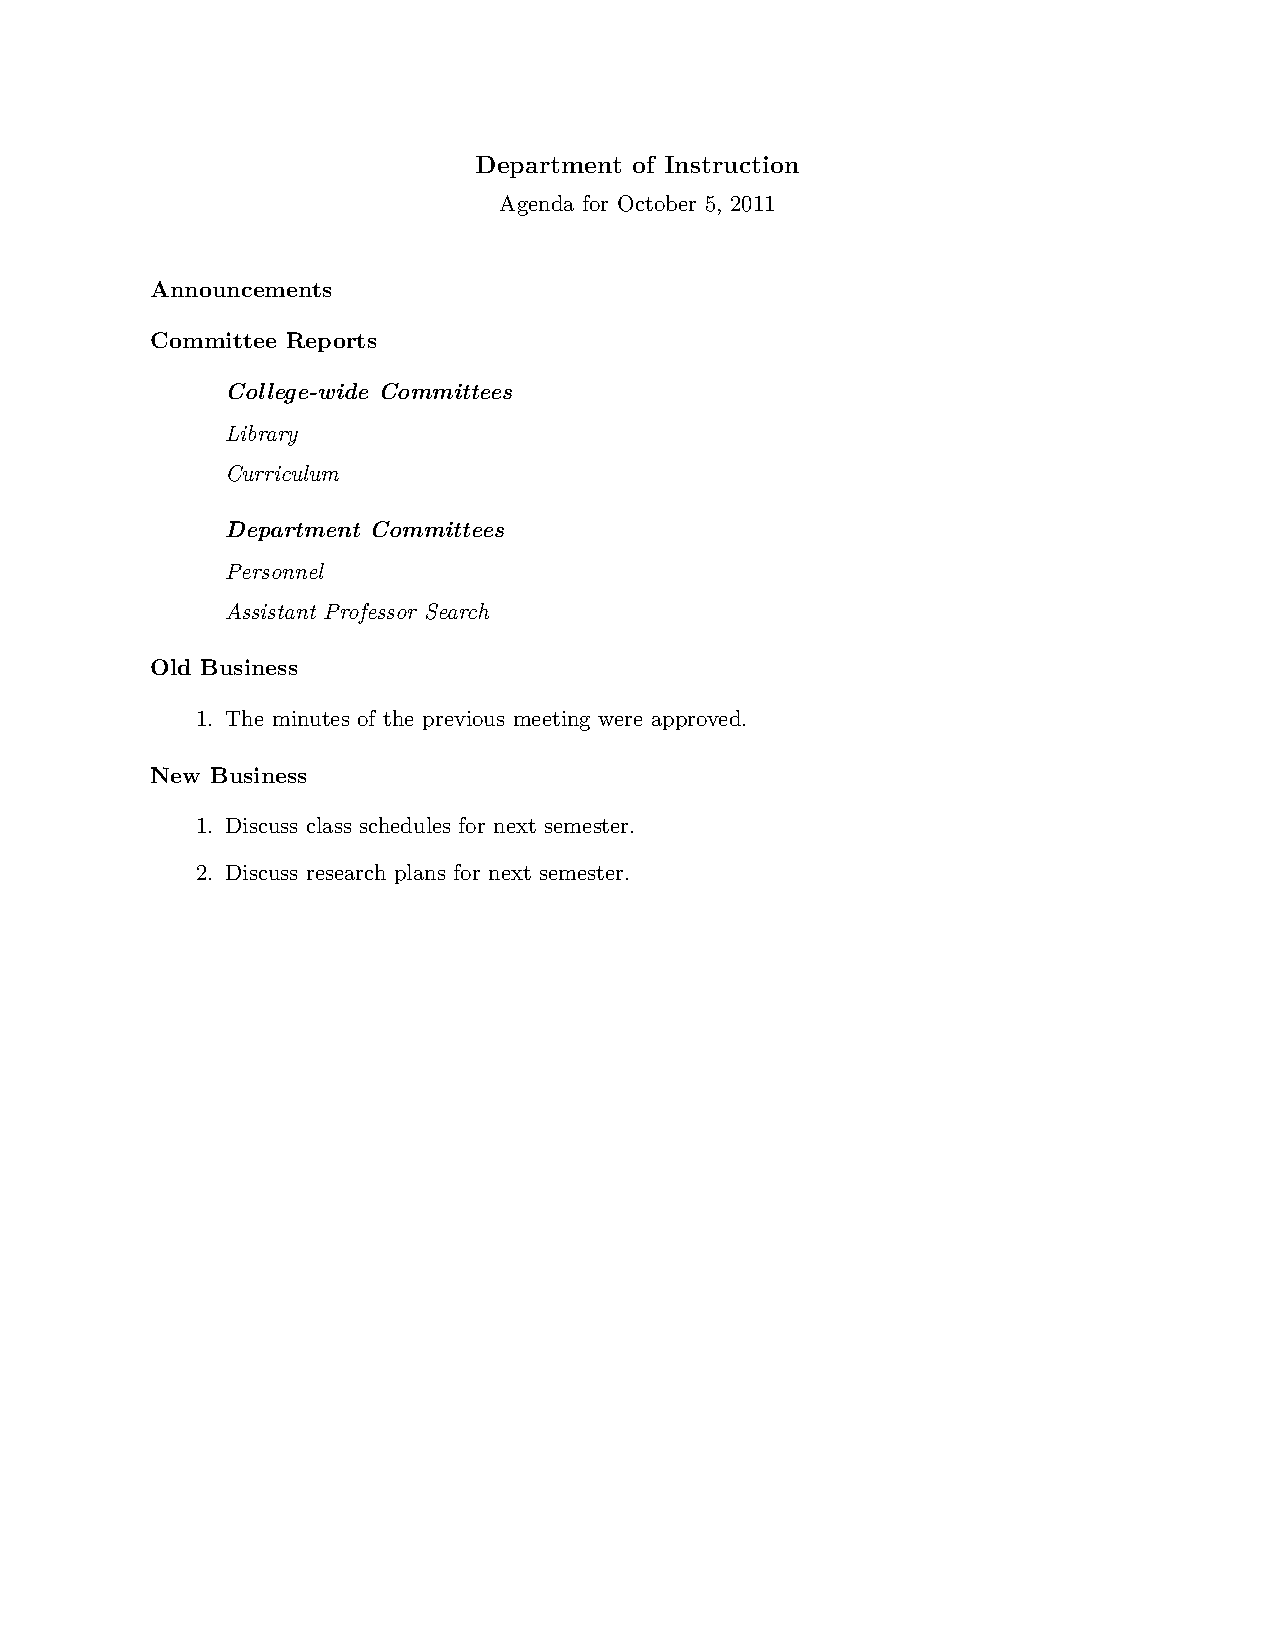
\includegraphics[scale=0.8, trim = 1in 1.5in 1in 0.8in]{samples/agenda.pdf}}%
%   {PRINTED AGENDA WILL BE DISPLAYED HERE \newpage}
%
% \subsection{Chair's Agenda (sample source code)}
%
% \begin{multicols*}{2}
% \begin{verbatim}
% \documentclass[11pt,chair]{meetingmins}
% 
% \setcommittee{Department of Instruction}
% 
% \setmembers{
%   \chair{B.~Smart},
%   B.~Brave,
%   D.~Claire,
%   B.~Gone
% }
% 
% \setdate{October 5, 2011}
% 
% \begin{document}
% \maketitle
% 
% \section{Announcements}
% \begin{hiddenitems}
% \item
% The dean is coming today.
% 
% \item
% The dean has canceled.
% 
% \end{hiddenitems}
% 
% \section{Committee Reports}
% 
% \subsection{College-wide Committees}
% \subsubsection{Library}
% 
% \subsubsection{Curriculum {\rm (D.~Claire)}}
% \begin{hiddensubitems}
% \item
% There is widespread interest in reforming
% the curriculum.
% 
% \item
% Unfortunately, no one seems interested
% in participating on the curriculum
% reform committee.
% \end{hiddensubitems}
% 
% \subsection{Department Committees}
% \subsubsection{Personnel}
% 
% \subsubsection{Assistant Professor Search}
% 
% 
%
%
% \section{Old Business}
% \begin{items}
% \item
% \priormins
% \end{items}
% 
% \section{New Business}
% \begin{items}
% \item
% Discuss class schedules for next semester.
% 
% \item
% Discuss research plans for next semester.
% \end{items}
% 
% \vspace{1em}
% \nextmeeting{Wednesday, October 19, at 3:00}
% 
% \end{document}
% \end{verbatim}
% \end{multicols*}
%
% \subsection{Chair's Agenda (printed version)}
% \IfFileExists{samples/chair.pdf}%
%   {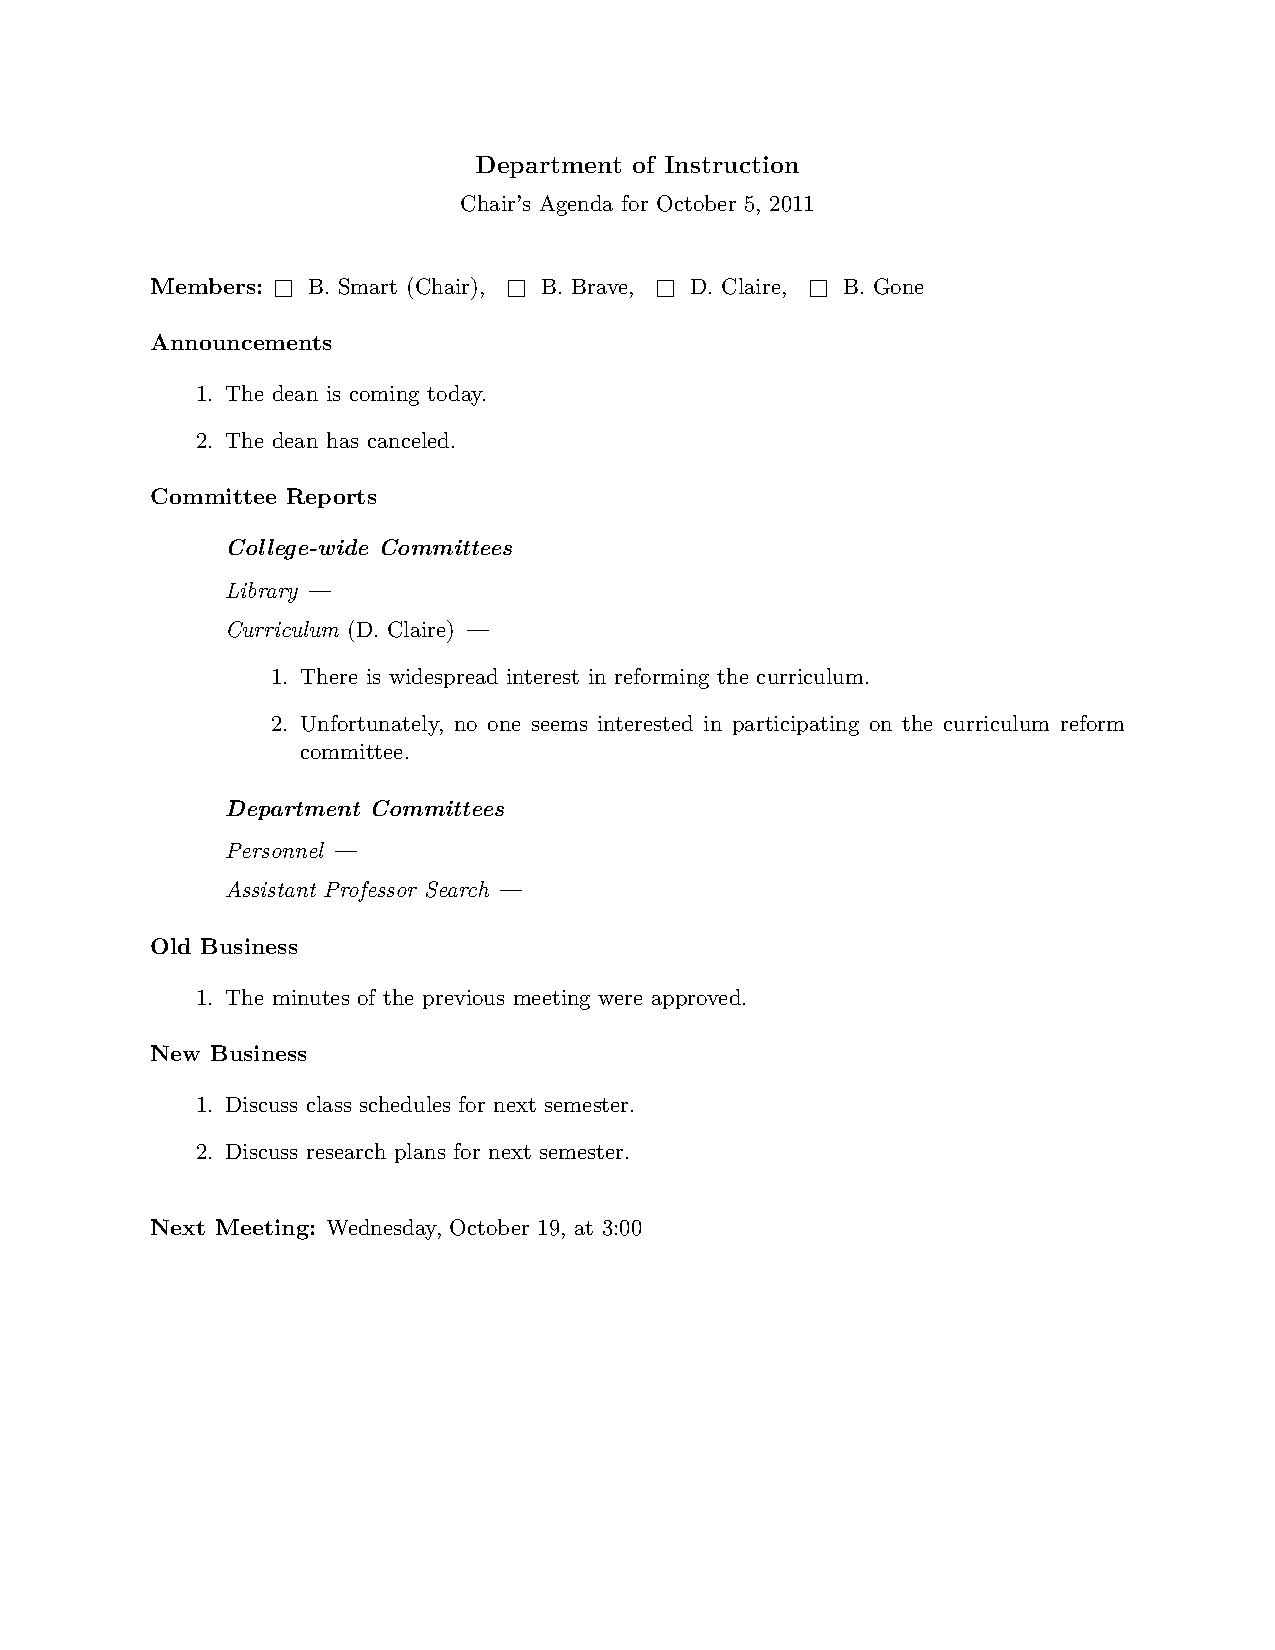
\includegraphics[scale=0.8, trim = 1in 1.5in 1in 0.8in]{samples/chair.pdf}}%
%   {PRINTED CHAIR'S AGENDA WILL BE DISPLAYED HERE \newpage}
%
% \subsection{Minutes (sample source code)}
%
% \begin{multicols*}{2}
% \begin{verbatim}
% \documentclass[11pt]{meetingmins}
% 
% \setcommittee{Department of Instruction}
% 
% \setmembers{
%   \chair{B.~Smart},
%   B.~Brave,
%   D.~Claire,
%   B.~Gone
% }
% 
% \setdate{October 5, 2011}
% 
% \setpresent{
%   \chair{B.~Smart},
%   B.~Brave,
%   D.~Claire
% }
% 
% \absent{B.~Gone \textit{(sabbatical)}}
% 
% \alsopresent{B.~There}
% 
% \begin{document}
% \maketitle
% 
% \section{Announcements}
% \begin{hiddenitems}
% \item
% The dean is coming today.
% 
% \item
% The dean has canceled.
% 
% \end{hiddenitems}
% 
% \section{Committee Reports}
% 
% \subsection{College-wide Committees}
% \subsubsection{Library}
% The library still has books that no one has read.
% 
% \subsubsection{Curriculum {\rm (D.~Claire)}}
% \begin{hiddensubitems}
% \item
% There is widespread interest in reforming
% the curriculum.
% 
% 
%
%
% \item
% Unfortunately, no one seems interested
% in participating on the curriculum
% reform committee.
% \end{hiddensubitems}
% 
% \subsection{Department Committees}
% \subsubsection{Personnel}
% 
% \subsubsection{Assistant Professor Search}
%
% \section{Old Business}
% \begin{items}
% \item
% \priormins
% \end{items}
% 
% \section{New Business}
% \begin{items}
% \item
% We will teach classes next semester.
% 
% \item
% We will do research next semester.
% \end{items}
% 
% \vspace{1em}
% \nextmeeting{Wednesday, October 19, at 3:00}
% 
% \end{document}
% \end{verbatim}
% \end{multicols*}
%
% \subsection{Minutes (printed version)}
% \IfFileExists{samples/minutes.pdf}%
%   {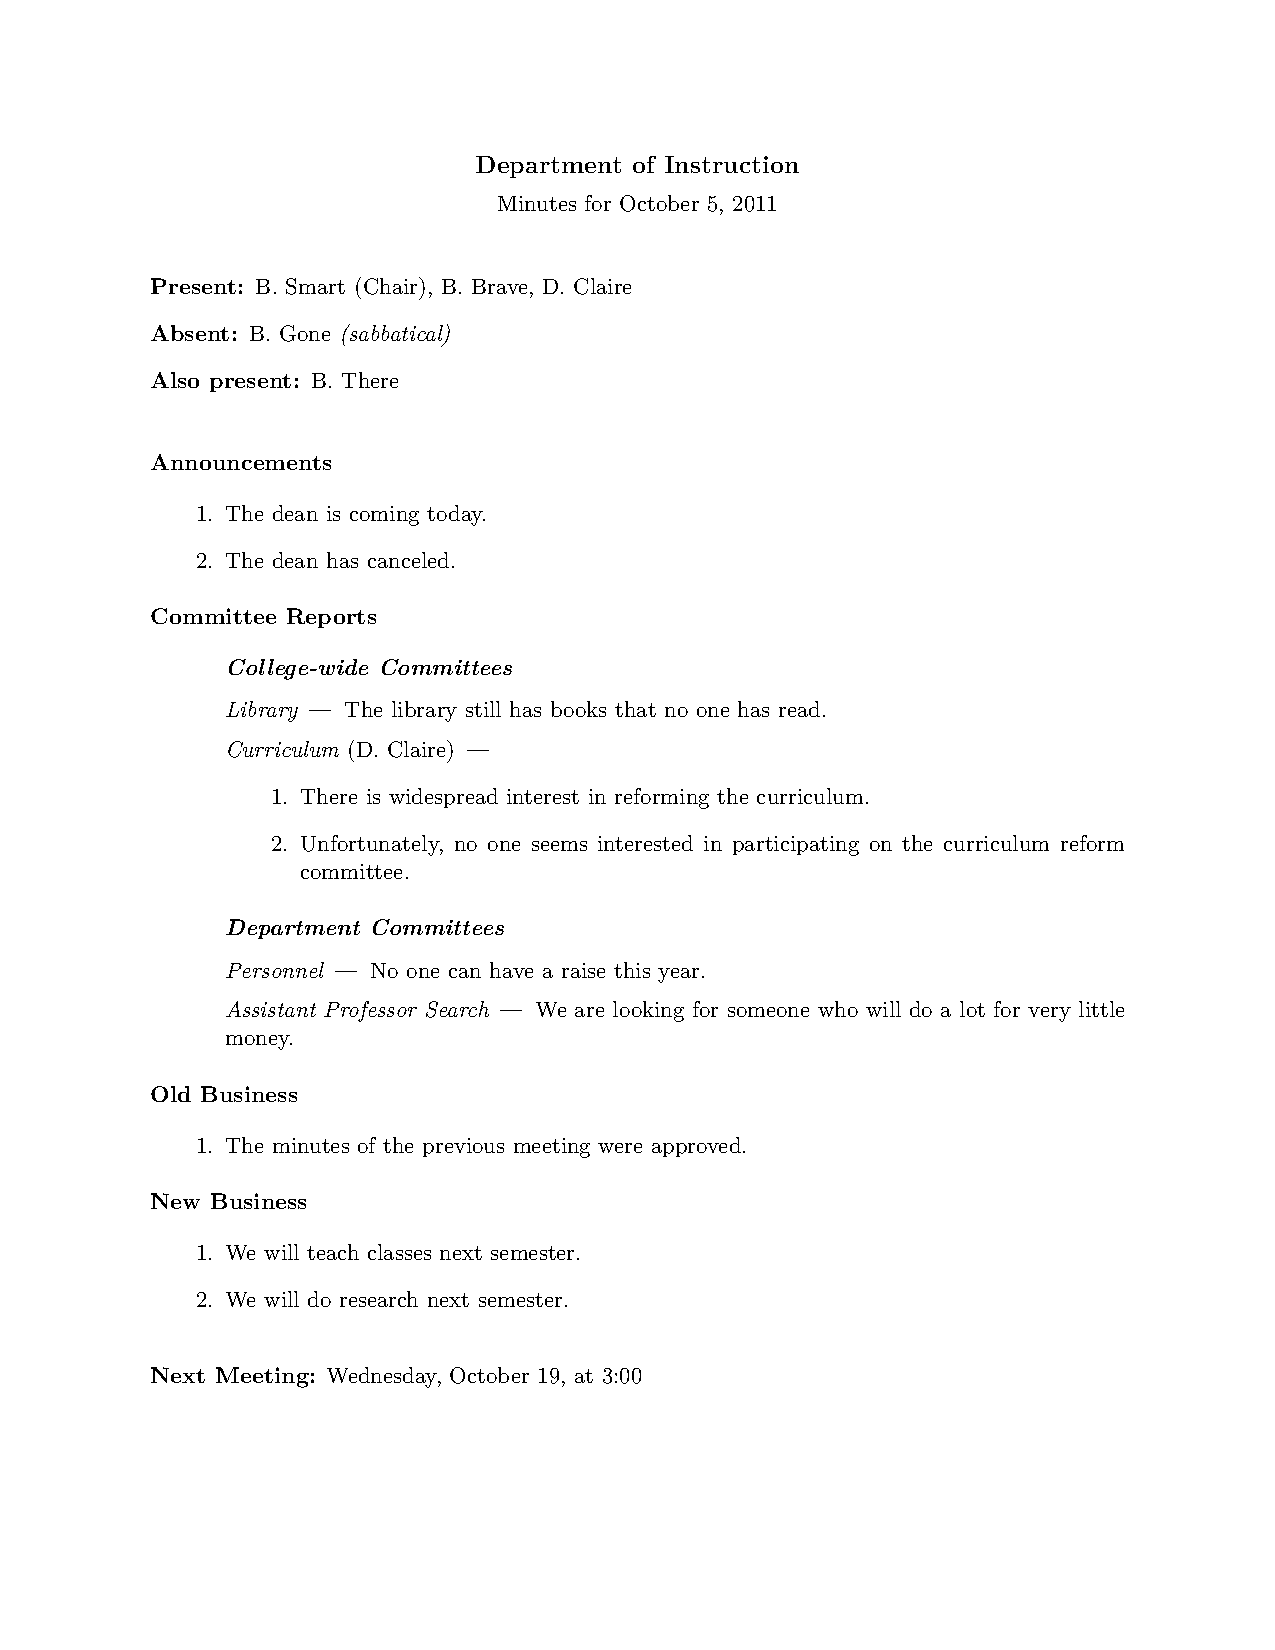
\includegraphics[scale=0.8, trim = 1in 1.5in 1in 0.8in]{samples/minutes.pdf}}%
%   {PRINTED MINUTES WILL BE DISPLAYED HERE \newpage}
%
%
%\StopEventually{^^A
%  \PrintChanges
%  \PrintIndex
%}
%
%    \begin{macrocode}
%<*class>
%    \end{macrocode}
%    
%\begin{macro}{\examplemacro}
%\changes{v1.0}{2009/10/06}{Some change from the previous version}
%    \begin{macrocode}
%
%

% specify whether this is an agenda or a minutes file
\DeclareOption{agenda}{%
\def\@agenda{\@agendamode}
}

% the chair's agenda has extra information on it
\DeclareOption{chair}{%
\def\@chair{\@chairmode}
}

% the notes option contains extra meeting notes that are not part of
% the official minutes
\DeclareOption{notes}{%
\def\@notes{\@notesmode}
}

% what group is meeting? 
\def\@committeename{}
\newcommand{\setcommittee}[1]{\def\@committee{#1}}
\newcommand{\show@committee}{\@committee}

% which persons are meeting?
\def\@members{None}
\newcommand{\setmembers}[1]{\def\@members{#1}}
\newcommand{\show@members}{\@members}

% what role do they have (e.g., chair)?
\newcommand{\role}[2]{#1~(#2)}
\newcommand{\chair}[1]{\role{#1}{Chair}}
\newcommand{\secretary}[1]{\role{#1}{Secretary}}

% who is absent? 
\global\let\@absent\@empty
\newcommand{\setabsent}[1]{\def\@absent{#1}}
\let\absent\setabsent %
\newcommand{\show@absent}{\@absent}

% who is present?
\global\let\@present\@empty
\newcommand{\setpresent}[1]{\def\@present{#1}}
\newcommand{\show@present}{\@present}

% who is also present?
\global\let\@alsopresent\@empty
\newcommand{\setalsopresent}[1]{\def\@alsopresent{#1}}
\let\alsopresent\setalsopresent %
\newcommand{\show@alsopresent}{\@alsopresent}

% what day is it?
\def\@date{\today}
\newcommand{\setdate}[1]{\def\@date{#1}}
\newcommand{\show@date}{\@date}


% Read all the documentclass options; pass them to article, unless the file
% named "<currentoption>.min" exists, in which case it is loaded
\DeclareOption*{\InputIfFileExists{\CurrentOption.min}{}{%
    \PassOptionsToClass{\CurrentOption}{article}}}

\ProcessOptions \relax

\LoadClass{article}


% Page layout
\RequirePackage[margin=1in]{geometry}

\RequirePackage[T1]{fontenc}
\RequirePackage{lmodern}


\RequirePackage{fancyhdr}
\fancypagestyle{firstpage}{%
  \fancyhf{} % clear all six fields
  \renewcommand{\headrulewidth}{0pt}
  \renewcommand{\footrulewidth}{0pt}
}
\fancypagestyle{followingpage}{%
  \fancyhf{} % clear all six fields
  \lhead{\show@committee, \show@date}
  \rhead{\thepage}
  \renewcommand{\headrulewidth}{1pt}
  \renewcommand{\footrulewidth}{0pt}
}

\pagestyle{followingpage}
\AtBeginDocument{\thispagestyle{firstpage}}


\RequirePackage{enumitem}

\@ifundefined{@chair}{% minutes/agenda
}{%  chair's agenda
  \RequirePackage{mathabx}
  \RequirePackage{xstring}
}


% material heading the minutes
\newcommand{\member@list}{
  \begin{description}
    \item[Members:] \show@members
  \end{description}
}

\newcommand{\member@table}{
  \begin{description}
    \raggedright
    \item[Members:] \StrSubstitute{$\Box$~\show@members}{,}{,\ \ \ $\Box$~}
  \end{description}  
}

\newcommand{\head@list}{
  \begin{description}
    \item[Present:] \show@present
    \ifx\@absent\@empty
      \relax
    \else
      \item[Absent:] \show@absent
    \fi %
    \ifx\@alsopresent\@empty
      \relax
    \else
      \item[Also present:] \show@alsopresent
    \fi %
  \end{description}
}

% maketitle
\renewcommand{\maketitle}{%
  \begin{center}
    {\large\textbf{\show@committee}}  \\[1ex]
    \@ifundefined{@agenda}{%
      \@ifundefined{@chair}{% minutes
        \@ifundefined{@notes}{% 
          Minutes for \show@date
        }{%  minutes with notes
          Notes for \show@date
        }
      }{%  chair's agenda
        Chair's Agenda for \show@date
      }%
    }{% agenda only
      Agenda for \show@date
    }%
  \end{center}
  \vspace{0.5ex}
  \@ifundefined{@agenda}{% minutes
    \@ifundefined{@chair}{% minutes
      \head@list
      \vspace{0.1ex}
    }{%  chair's agenda
      \member@table
    }
  }{% agenda only
%    \member@list
%    \vspace{1pt}
  }
}{%
}


% section formatting
\setcounter{secnumdepth}{0}
\renewcommand{\section}{\@startsection {section}{1}{\z@}%
    {1\baselineskip \@plus 0.2ex \@minus 0.2ex\leftskip=0in}%
    {0.8\baselineskip \@plus .2ex}%
    {\normalfont\normalsize\bfseries}}
\renewcommand{\subsection}{\@startsection{subsection}{2}{0.5in}%
    {1\baselineskip \@plus 0.2ex \@minus 0.2ex\leftskip=0in}%
    {0.5\baselineskip \@plus 0.2ex}%
    {\normalfont\normalsize\bfseries\itshape}}

\@ifundefined{@agenda}{%
  \@ifundefined{@chair}{% minutes
    \renewcommand{\subsubsection}[1]{\@startsection{subsubsection}{3}{0in}%
      {0.4\baselineskip \@plus 0.2ex \@minus 0.2ex\leftskip=0.5in}%
      {-\z@}%
      {\normalfont\normalsize\itshape}{#1} \hspace{0.2em} ---\hspace{0.2em}}
  }{% chair's agenda
    \renewcommand{\subsubsection}[1]{\@startsection{subsubsection}{3}{0in}%
      {0.4\baselineskip \@plus 0.2ex \@minus 0.2ex\leftskip=0.5in}%
      {-\z@}%
      {\normalfont\normalsize\itshape}{#1} \hspace{0.2em} ---\hspace{0.2em}}
  }
}{% agenda only
  \renewcommand{\subsubsection}[1]{\@startsection{subsubsection}{3}{0in}%
    {0.4\baselineskip \@plus 0.2ex \@minus 0.2ex\leftskip=0.5in}%
    {-\z@}%
    {\normalfont\normalsize\itshape}{#1}}
}

\RequirePackage{environ}

\newenvironment{emptysection}{\Collect@Body\@gobble}{}

% top-level items (under \section commands)
\newenvironment{items}{%
  \begin{itemlist}
}{%
  \end{itemlist}
}

\newenvironment{itemlist}{%
  \begin{enumerate}[leftmargin=0.5in]
}{%
  \end{enumerate}
}

\@ifundefined{@agenda}{% minutes
  \newenvironment{hiddenitems}{\begin{enumerate}[leftmargin=0.5in]}{\end{enumerate}}
}{% agenda only
  \let\hiddenitems\emptysection
}


\@ifundefined{@agenda}{% minutes
  \newenvironment{hiddentext}{}{}
}{% agenda only
  \let\hiddentext\emptysection
}


% second-level items (under \subsection commands)
\newenvironment{subitems}{%
  \begin{subitemlist}
}{%
  \end{subitemlist}
}

\newenvironment{subitemlist}{%
  \begin{enumerate}[leftmargin=1in]
}{%
  \end{enumerate}
}

\@ifundefined{@agenda}{% minutes
  \newenvironment{hiddensubitems}{\begin{enumerate}[leftmargin=1in]}{\end{enumerate}}
}{% agenda only
  \let\hiddensubitems\emptysection
}


% third-level items (under \subsubsection commands)
\newenvironment{subsubitems}{%
  \begin{subsubitemlist}
}{%
  \end{subsubitemlist}
}

\newenvironment{subsubitemlist}{%
  \begin{enumerate}[leftmargin=1in]
}{%
  \end{enumerate}
}

\@ifundefined{@agenda}{% minutes
  \newenvironment{hiddensubsubitems}{\begin{enumerate}[leftmargin=1in]}{\end{enumerate}}
}{% agenda only
  \let\hiddensubsubitems\emptysection
}


% Statement of approval of previous minutes
\newcommand{\priormins}{The minutes of the previous meeting were approved.}


% when is the next meeting?
\newcommand{\nextmeeting}[1]{%
  \@ifundefined{@agenda}{% minutes
    \par\noindent\textbf{Next Meeting:} #1\par
  }{% agenda only
    %\par\noindent\textbf{Next Meeting:} #1\par
  }
}

%    \end{macrocode}
%\end{macro} 
%
%    \begin{macrocode}
%</class>
%    \end{macrocode}
%
%
% %%%%%%%%%%%  SAMPLE FILES  %%%%%%%%%%%%
%
%\begin{macro}{department.min}
%    \begin{macrocode}
%<*sampledepartment>

\setcommittee{Department of Instruction}

\setmembers{
  \chair{B.~Smart},
  B.~Brave,
  D.~Claire,
  B.~Gone
}

%</sampledepartment>
%    \end{macrocode}
%\end{macro} 
%
%\begin{macro}{agenda.tex}
%    \begin{macrocode}
%<*agenda>
\documentclass[11pt,agenda]{meetingmins}

%% Optionally, the following text could be set in the file
%% department.min in this folder, then add the option 'department'
%% in the \documentclass line of this .tex file:
%%\setcommittee{Department of Instruction}
%%
%%\setmembers{
%%  \chair{B.~Smart},
%%  B.~Brave,
%%  D.~Claire,
%%  B.~Gone
%%}

\setcommittee{Department of Instruction}

\setmembers{
  \chair{B.~Smart},
  B.~Brave,
  D.~Claire,
  B.~Gone
}

\setdate{October 5, 2011}

\begin{document}
\maketitle

\section{Announcements}
\begin{hiddenitems}
\item
The dean is coming today.

\item
The dean has canceled.

\end{hiddenitems}

\section{Committee Reports}

\subsection{College-wide Committees}
\subsubsection{Library}

\subsubsection{Curriculum}
\begin{hiddensubitems}
\item
There is widespread interest in reforming the curriculum.

\item
Unfortunately, no one seems interested in participating on the
curriculum reform committee.
\end{hiddensubitems}

\subsection{Department Committees}
\subsubsection{Personnel}

\subsubsection{Assistant Professor Search}

\section{Old Business}
\begin{items}
\item
\priormins
\end{items}

\section{New Business}
\begin{items}
\item
Discuss class schedules for next semester.

\item
Discuss research plans for next semester.
\end{items}

\vspace{1em}
\nextmeeting{Wednesday, October 19, at 3:00}

\end{document}
%</agenda>
%    \end{macrocode}
%\end{macro} 
%
%
%
%\begin{macro}{chair.tex}
%    \begin{macrocode}
%<*chair>
\documentclass[11pt,chair]{meetingmins}

%% Optionally, the following text could be set in the file
%% department.min in this folder, then add the option 'department'
%% in the \documentclass line of this .tex file:
%%\setcommittee{Department of Instruction}
%%
%%\setmembers{
%%  \chair{B.~Smart},
%%  B.~Brave,
%%  D.~Claire,
%%  B.~Gone
%%}

\setcommittee{Department of Instruction}

\setmembers{
  \chair{B.~Smart},
  B.~Brave,
  D.~Claire,
  B.~Gone
}

\setdate{October 5, 2011}

\begin{document}
\maketitle

\section{Announcements}
\begin{hiddenitems}
\item
The dean is coming today.

\item
The dean has canceled.

\end{hiddenitems}

\section{Committee Reports}

\subsection{College-wide Committees}
\subsubsection{Library}

\subsubsection{Curriculum {\rm (D.~Claire)}}
\begin{hiddensubitems}
\item
There is widespread interest in reforming the curriculum.

\item
Unfortunately, no one seems interested in participating on the
curriculum reform committee.
\end{hiddensubitems}

\subsection{Department Committees}
\subsubsection{Personnel}

\subsubsection{Assistant Professor Search}

\section{Old Business}
\begin{items}
\item
\priormins
\end{items}

\section{New Business}
\begin{items}
\item
Discuss class schedules for next semester.

\item
Discuss research plans for next semester.
\end{items}

\vspace{1em}
\nextmeeting{Wednesday, October 19, at 3:00}

\end{document}
%</chair>
%    \end{macrocode}
%\end{macro} 
%
%
%
%\begin{macro}{minutes.tex}
%    \begin{macrocode}
%<*minutes>
\documentclass[11pt]{meetingmins}

%% Optionally, the following text could be set in the file
%% department.min in this folder, then add the option 'department'
%% in the \documentclass line of this .tex file:
%%\setcommittee{Department of Instruction}
%%
%%\setmembers{
%%  \chair{B.~Smart},
%%  B.~Brave,
%%  D.~Claire,
%%  B.~Gone
%%}

\setcommittee{Department of Instruction}

\setmembers{
  \chair{B.~Smart},
  B.~Brave,
  D.~Claire,
  B.~Gone
}

\setdate{October 5, 2011}

\setpresent{
  \chair{B.~Smart},
  B.~Brave,
  D.~Claire
}

\absent{B.~Gone \textit{(sabbatical)}}

\alsopresent{B.~There}

\begin{document}
\maketitle

\section{Announcements}
\begin{hiddenitems}
\item
The dean is coming today.

\item
The dean has canceled.

\end{hiddenitems}

\section{Committee Reports}

\subsection{College-wide Committees}
\subsubsection{Library}
The library still has books that no one has read.

\subsubsection{Curriculum {\rm (D.~Claire)}}
\begin{hiddensubitems}
\item
There is widespread interest in reforming the curriculum.

\item
Unfortunately, no one seems interested in participating on the
curriculum reform committee.
\end{hiddensubitems}

\subsection{Department Committees}
\subsubsection{Personnel}
No one can have a raise this year.

\subsubsection{Assistant Professor Search}
We are looking for someone who will do a lot for very little money.

\section{Old Business}
\begin{items}
\item
\priormins
\end{items}

\section{New Business}
\begin{items}
\item
We will teach classes next semester.

\item
We will do research next semester.
\end{items}

\vspace{1em}
\nextmeeting{Wednesday, October 19, at 3:00}

\end{document}
%</minutes>
%    \end{macrocode}
%\end{macro} 
%
%
%\Finale